\section{Assignment description}
The second assignment of Modeling and Control of Manipulators focuses on manipulators' geometry and direct kinematics. 

\begin{itemize}
    \item Download the .zip file called \textit{template\_MATLAB-assignment2} from the Aulaweb page of this course.
    \item Implement the code to solve the exercises on MATLAB by filling the template classes called \textit{geometricModel} and \textit{kinematicModel}
    \item Write a report motivating your answers, following the predefined format on this document.
\end{itemize}

\subsection{Exercise 1}
 Given the following CAD model of an industrial 7 DoF manipulator:
 
\textbf{Q1.1} Define all the model matrices, by filling the structures in the \textit{BuildTree()} function. Be careful to define the z-axis coinciding with the joint rotation axis, and such that the positive rotation is the same as showed in the CAD model you received. Draw on the CAD model the reference frames for each link and insert it into the report.

\textbf{Q1.2} Implement the method of \textit{geometricModel} called \textit{updateDirectGeometry()} which should compute the model matrices as a function of the joint position $q$. Explain the method used and comment on the results obtained.

\textbf{Q1.3} Implement the method of \textit{geometricModel} called \textit{getTransformWrtBase()} which should compute the transformation matrix from the base to a given frame. Calculate the following transformation matrices: $^b_e T$, $^5_3 T$. Explain the method used and comment on the results obtained.

\textbf{Q1.4} Implement the method of \textit{kinematicModel} called \textit{updateJacobian()} which should compute the jacobian of a given geometric model considering the possibility of having \textit{rotational} or \textit{prismatic} joints. Compute the Jacobian matrix of the manipulator for the end-effector. Explain the method used and comment on the results obtained.

\textit{Remark:} The methods should be implemented for a generic serial manipulator. For instance, joint types, and the number of joints should be parameters. 

\newpage

\begin{figure} [ht]
\centering
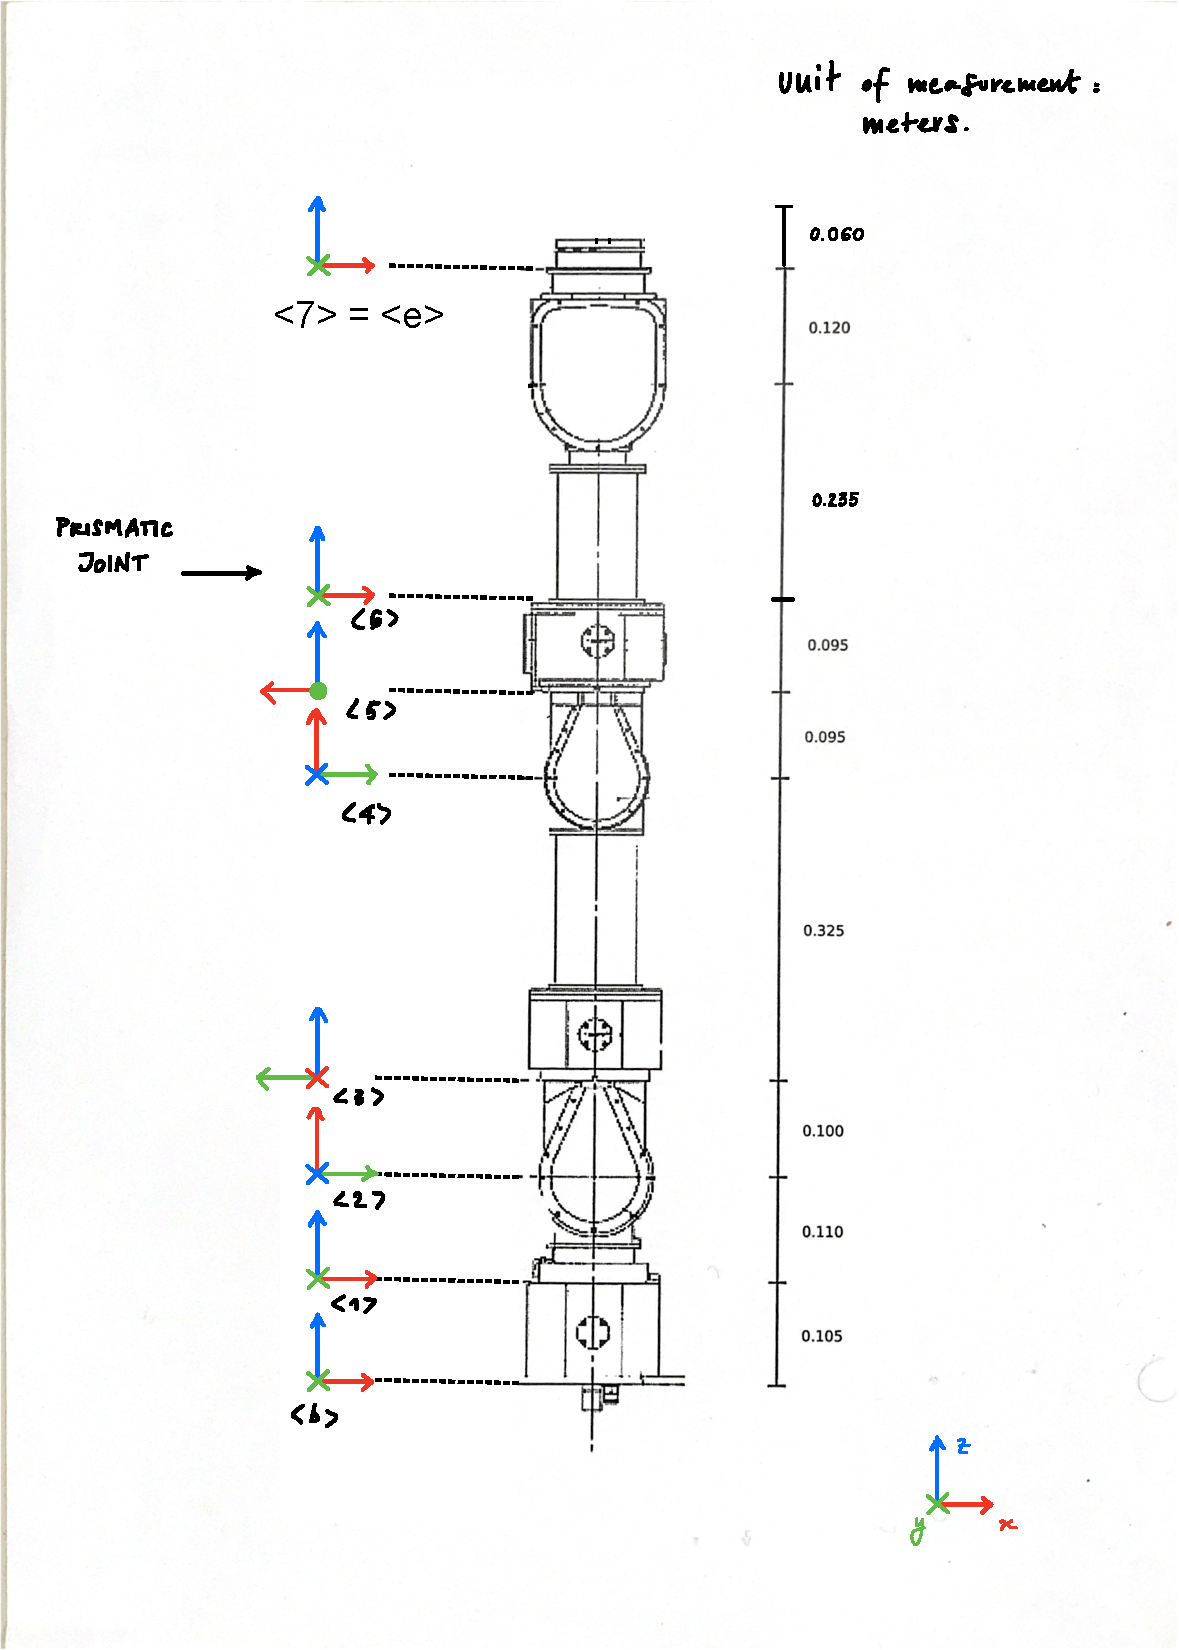
\includegraphics[width=\textwidth*8/10]{Resources/cad_model-1.pdf}
\caption{CAD model of the robot}
\label{fig:ex2}
\end{figure}

\newpage